\documentclass[../../main.tex]{subfiles}
\begin{document}

{\bf [解答]}

複素数平面上で点 $P_n(x_n, y_n)$ に対応する複素数を $z_n = x_n + i y_n$ とする．
与えられた漸化式
\begin{align}
  \begin{cases}
    x_{n+1} = ax_n - by_n \\
    y_{n+1} = bx_n + ay_n \\
    x_0=1, y_0=0
  \end{cases} \label{eq:1}
\end{align}
は，複素数表現で
\begin{align}
  x_{n+1}+iy_{n+1} = (a+bi)(x_n+iy_n) \quad (n = 0, 1, 2, \dots)
\end{align}
と表される．$z_0 = x_0 + i y_0 = 1$ であるから，一般項は
\begin{align}
  x_{n}+iy_{n} = (a+bi)^n \quad (n = 0, 1, 2, \dots) \label{eq:2}
\end{align}
となる．ここで$e(\theta)=\cos\theta+i\sin\theta$として実数$r\ge 0$を用いて
\begin{align}
  a+bi = re(\theta) \label{eq:3}
\end{align}
とおくと，\cref{eq:2}より
\begin{align}
  x_{n}+iy_{n} = r^ne(n\theta) \label{eq:4}
\end{align}
である．

条件 (i) より$x_n+iy_n=x_0+iy_0=1$だから \cref{eq:4}で絶対値と偏角を比較して
\begin{align}
  \begin{cases}
    r^6 = 1 \implies r = 1 \\
    6\theta = 2k\pi \quad (k \in \mathbb{Z}) \implies \theta = \dfrac{k\pi}{3} \quad (k=0,1,\cdots,5)
  \end{cases} \label{eq:5}
\end{align}
である．ただし，最後$0 \le \theta < 2\pi$で考えて良いので$k$の範囲を絞った．

% TODO: k=1,5の時の単位円上のP_iの位置
\begin{figure}[htbp]
  \centering
  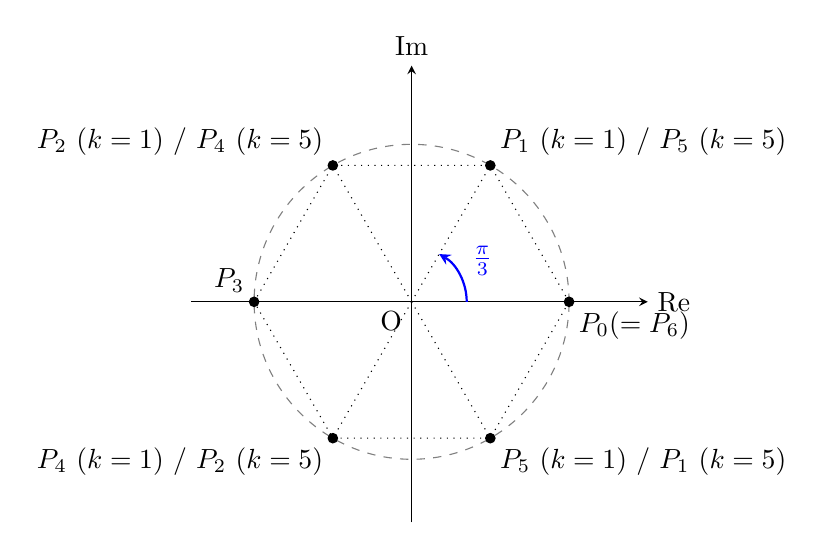
\begin{tikzpicture}[scale=2, >=stealth]
    % 座標軸
    \draw[->] (-1.4, 0) -- (1.5, 0) node[right] {$\mathrm{Re}$};
    \draw[->] (0, -1.4) -- (0, 1.5) node[above] {$\mathrm{Im}$};
    \node[below left] at (0, 0) {$\mathrm{O}$};

    % 単位円
    \draw[dashed, gray] (0,0) circle (1);

    % 正六角形のガイド線
    \draw[dotted, black] (0:1) -- (60:1) -- (120:1) -- (180:1) -- (240:1) -- (300:1) -- cycle;
    \draw[dotted, black] (0:0) -- (60:1);
    \draw[dotted, black] (0:0) -- (120:1);
    \draw[dotted, black] (0:0) -- (180:1);
    \draw[dotted, black] (0:0) -- (240:1);
    \draw[dotted, black] (0:0) -- (300:1);

    % 各頂点（P_i）のプロット
    % k=1のとき反時計回り、k=5のとき時計回りに対応
    \filldraw (0:1) circle (0.03) node[below right] {$P_0 (=P_6)$};
    \filldraw (60:1) circle (0.03) node[above right] {$P_1$ ($k=1$) / $P_5$ ($k=5$)};
    \filldraw (120:1) circle (0.03) node[above left] {$P_2$ ($k=1$) / $P_4$ ($k=5$)};
    \filldraw (180:1) circle (0.03) node[above left] {$P_3$};
    \filldraw (240:1) circle (0.03) node[below left] {$P_4$ ($k=1$) / $P_2$ ($k=5$)};
    \filldraw (300:1) circle (0.03) node[below right] {$P_5$ ($k=1$) / $P_1$ ($k=5$)};

    % 偏角の矢印（k=1）
    \draw[->, thick, blue] (0.35, 0) arc (0:60:0.35);
    \node[blue] at (30:0.52) {$\frac{\pi}{3}$};
  \end{tikzpicture}
  \caption{$k=1, 5$ における単位円上の点 $P_n$ の配置}
  \label{fig:points}
\end{figure}

次に条件 (ii) について考えると，$x_n+iy_n$が$n=0,1,\cdots,5$に対して全て相異なれば良い．
$k=0,1,\cdots,5$に対して個別で考えると
\begin{itemize}
  \item $k=0$: $P_0=P_1$となり不適．
  \item $k=1$: $P_i$は全て異なり適する．
  \item $k=2$: $P_0=P_3$となり不適．
  \item $k=3$: $P_0=P_2$となり不適．
  \item $k=4$: $P_0=P_3$となり不適．
  \item $k=5$: $P_i$は全て異なり適する．
\end{itemize}
だから求めるのは$k=1,5$の時で
\begin{align}
  a+bi = \dfrac{1}{2}\pm \dfrac{\sqrt{3}}{2}i \quad
  \therefore
  (a,b) = \left(\dfrac{1}{2},\pm\dfrac{\sqrt{3}}{2}\right)
\end{align}
である．

{\bf [別解]}

後半は個別の$k$について検討しなくても以下のような議論も可能だ．
要するに$n=0,1,\cdots,5$に対して$e(n\theta)$が互いに異なれば良い．
\cref{eq:5}を代入して$e(\dfrac{ik\pi}{3})$たちが全て相異なるためには，
$k$が$6$と互いに素でなければならない．
すなわち，
\begin{align}
  k = 1, 5
\end{align}
である．

\end{document}
